\begin{figure}[tb]
\centering
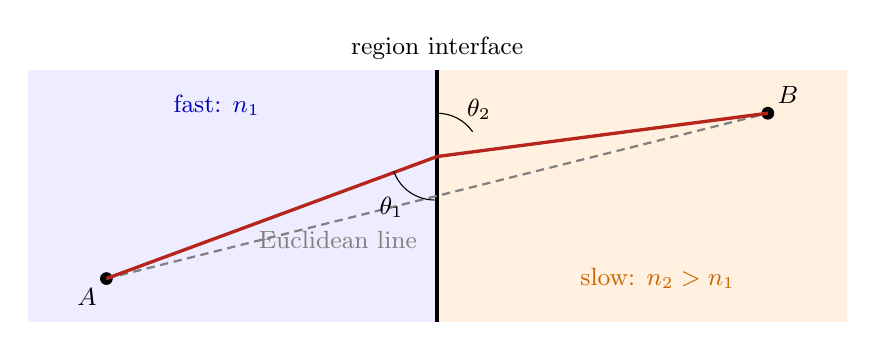
\begin{tikzpicture}[font=\small,x=1cm,y=1cm]
 \fill[blue!7] (0,0) rectangle (5.2,3.2);
 \fill[orange!12] (5.2,0) rectangle (10.4,3.2);
 \draw[very thick] (5.2,0)--(5.2,3.2) node[above] {region interface};
 \fill (1,.55) circle (2.3pt) node[below left] {$A$};
 \fill (9.4,2.65) circle (2.3pt) node[above right] {$B$};
 \draw[gray,densely dashed,thick] (1,.55)--(9.4,2.65) node[pos=.35,below] {Euclidean line};
 \draw[BrickRed,very thick] (1,.55)--(5.2,2.1)--(9.4,2.65);
 \draw[dotted] (5.2,1.2)--(5.2,2.9);
 \draw (4.65,1.91) arc[start angle=200,end angle=270,radius=.55];
 \draw (5.2,2.1) ++(0,.55) arc[start angle=90,end angle=35,radius=.55];
 \node at (4.62,1.45) {$\theta_1$};
 \node at (5.73,2.7) {$\theta_2$};
 \node[blue!70!black] at (2.4,2.75) {fast: $n_1$};
 \node[orange!80!black] at (8.0,.55) {slow: $n_2>n_1$};
\end{tikzpicture}
\caption{Piecewise-flat teaching model.  A path can be longer in amperes but
faster in time by spending more distance in the dynamically fast region.
Stationarity of the interface crossing gives the Snell condition.}
\label{fig:optical-pwa}
\end{figure}

